\documentclass[fleqn,answers,addpoints]{exam}

%\usepackage{graphicx, fancyhdr}
\usepackage{etoolbox}
\usepackage{subcaption}
\usepackage{etoolbox}
\usepackage{tikz,pgfplots}
\usepackage{amsmath, amsfonts}
\usepackage{color}

%% For LaTeX-Box: root = stat105_exam1_info.tex 
%%%%%%%%%%%%%%%%%%%%%%%%%%%%%%%%%%%%%%%%%%%%%%%%%%%%%%%%%%%%%%%%%%%%%%%%%%%%%%%%
%  File Name: stat105_exam1_info.tex
%  Purpose:
%
%  Creation Date: 24-09-2015
%  Last Modified: Thu Sep 24 13:51:36 2015
%  Created By:
%%%%%%%%%%%%%%%%%%%%%%%%%%%%%%%%%%%%%%%%%%%%%%%%%%%%%%%%%%%%%%%%%%%%%%%%%%%%%%%%
\newcommand{\course}[1]{\ifstrempty{#1}{STAT 105}{STAT 105, Section #1}}
\newcommand{\sectionNumber}{B}
\newcommand{\examDate}{October 1, 2015}
\newcommand{\semester}{FALL 2015}
\newcommand{\examNumber}{II}

\newcommand{\examTitle}{Exam \examNumber}

\runningheader{\course{\sectionNumber}}{Exam \examNumber}{\examDate}
\runningfooter{}{}{Page \thepage of \numpages}

\newcommand{\examCoverPage}{
   \begin{coverpages}
   \centering
   {\bfseries\scshape\Huge Exam I \par}
   \vspace{1cm}
   {\bfseries\scshape\LARGE \course{\sectionNumber} \par}
   {\bfseries\scshape\LARGE \semester \par}

   \vspace{2cm}

   \fbox{\fbox{\parbox{5.5in}{\centering 

      \vspace{.25cm} 
      
      {\bfseries\Large Instructions} \\

      \vspace{.5cm} 

      \begin{itemize}
         \item  The exam is scheduled for 80 minutes, from 8:00 to 9:20 AM. At 9:20 AM the exam will end.\\
         \item  A forumula sheet is attached to the end of the exam. Feel free to tear it off.\\
         \item  You may use a calculator during this exam.\\
         \item  Answer the questions in the space provided. If you run out of room, continue on the back of the page. \\
         \item  If you have any questions about, or need clarification on the meaning of an item on this exam, please ask your instructor. No other form of external help is permitted attempting to receive help or provide help to others will be considered cheating.\\
         \item  {\bfseries Do not cheat on this exam.} Academic integrity demands an honest and fair testing environment. Cheating will not be tolerated and will result in an immediate score of 0 on the exam and an incident report will be submitted to the dean's office.\\
      \end{itemize}

   }}}

   \vspace{2cm}

   \makebox[0.6\textwidth]{Name:\enspace\hrulefill}

   \vspace{1cm}

   \makebox[0.6\textwidth]{Student ID:\enspace\hrulefill}
   \end{coverpages}

}


\newcommand{\course}[1]{\ifstrempty{#1}{STAT 305}{STAT 305, Section #1}}
\newcommand{\sectionNumber}{B}
\newcommand{\examDate}{April 11, 2019}
\newcommand{\semester}{Spring 2019}
\newcommand{\examNumber}{II}
\newcommand{\qparts}[1]{\begin{parts} #1 \end{parts}}
\newcommand{\qitems}[1]{\begin{itemize} #1 \end{itemize}}

% Document definitions
\newcommand{\examTitle}{Exam \examNumber}
\runningheader{\course{\sectionNumber}}{Exam \examNumber}{\examDate}
\runningfooter{}{}{Page\ \thepage\ of\ \numpages}

\begin{document}

\begin{coverpages}
   \centering
   {\bfseries\scshape\Huge Exam \examNumber \par}
   \vspace{1cm}
   {\bfseries\scshape\LARGE \course{\sectionNumber} \par}
   {\bfseries\scshape\LARGE \semester \par}
   \vspace{2cm}
   \fbox{\fbox{\parbox{5.5in}{
      \centering 
      \vspace{.25cm} 
      {\bfseries\Large Instructions} \\
      \vspace{.25cm} 
      \begin{itemize}
         \item  The exam is scheduled for 80 minutes, from 3:40 to 5:00 PM. At 5:00 PM the exam will end.\\
         \item  A forumula sheet is attached to the end of the exam. Feel free to tear it off.\\
         \item  You are allowed to use a self-produced one-page (front and back) formula sheet during this exam.\\
         \item  You may use a calculator during this exam.\\
         \item  Answer the questions in the space provided. If you run out of room, continue on the back of the page. \\
         \item  If you have any questions about, or need clarification on the meaning of an item on this exam, please ask your instructor. No other form of external help is permitted attempting to receive help or provide help to others will be considered cheating.\\
         \item  {\bfseries Do not cheat on this exam.} Academic integrity demands an honest and fair testing environment. Cheating will not be tolerated and will result in an immediate score of 0 on the exam and an incident report will be submitted to the office of the dean.\\
      \end{itemize}
   }}}
   \vspace{1cm}
   \makebox[0.6\textwidth]{}
   \vspace{1cm}
   \makebox[0.6\textwidth]{Name:\enspace\hrulefill}
   \vspace{1cm}
   \makebox[0.6\textwidth]{Student ID:\enspace\hrulefill}
\end{coverpages}

\begin{questions}

\question[2] For continuous distributions, the probability density
function is \fillin~continuous and the cumulative density function is
\fillin~continuous.

\begin{oneparchoices}
\choice \textbf{always} and \textbf{always}
\choice \textbf{always} and \textbf{sometimes}
\choice \textbf{sometimes} and \textbf{always}
\choice \textbf{sometimes} and \textbf{sometimes}
\end{oneparchoices}
\vspace{1cm}

\question[3]Circle the name of the distribution which best matches the
plot of the \textbf{probability density function}:

\begin{center}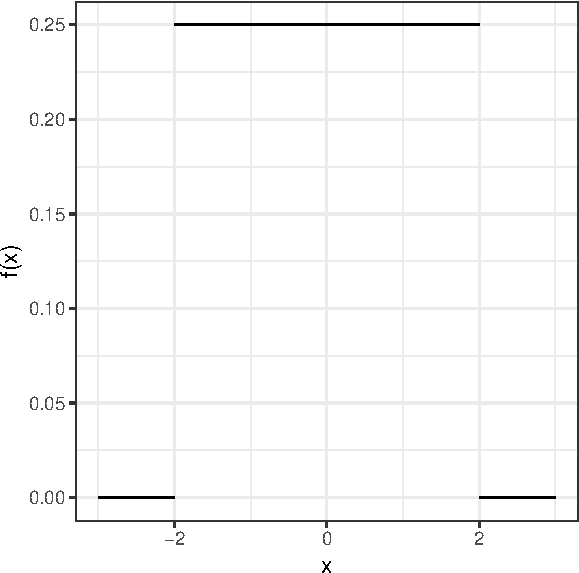
\includegraphics[width=.4\linewidth,height=.4\linewidth]{stat305-exam2_files/figure-latex/unnamed-chunk-3-1} \end{center}
\begin{oneparchoices}
\choice standard normal
\choice normal 
\choice exponential 
\choice poisson
\choice uniform
\end{oneparchoices}

\question[3]Circle the name of the distribution which best matches the
plot of the \textbf{cumulative density function}:

\begin{center}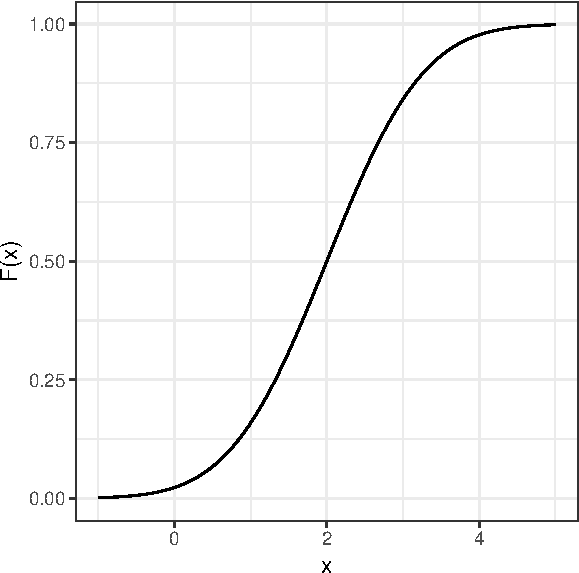
\includegraphics[width=.4\linewidth,height=.4\linewidth]{stat305-exam2_files/figure-latex/unnamed-chunk-4-1} \end{center}
\begin{oneparchoices}
\choice standard normal
\choice normal 
\choice exponential 
\choice binomial
\choice uniform
\end{oneparchoices}
\vspace{1cm}

\newpage

\question[4] The left plot depicts the \textbf{cumulative density
function} of a random variable \(X\). In the plot on the right, sketch
the corresponding probability density function.

\begin{center}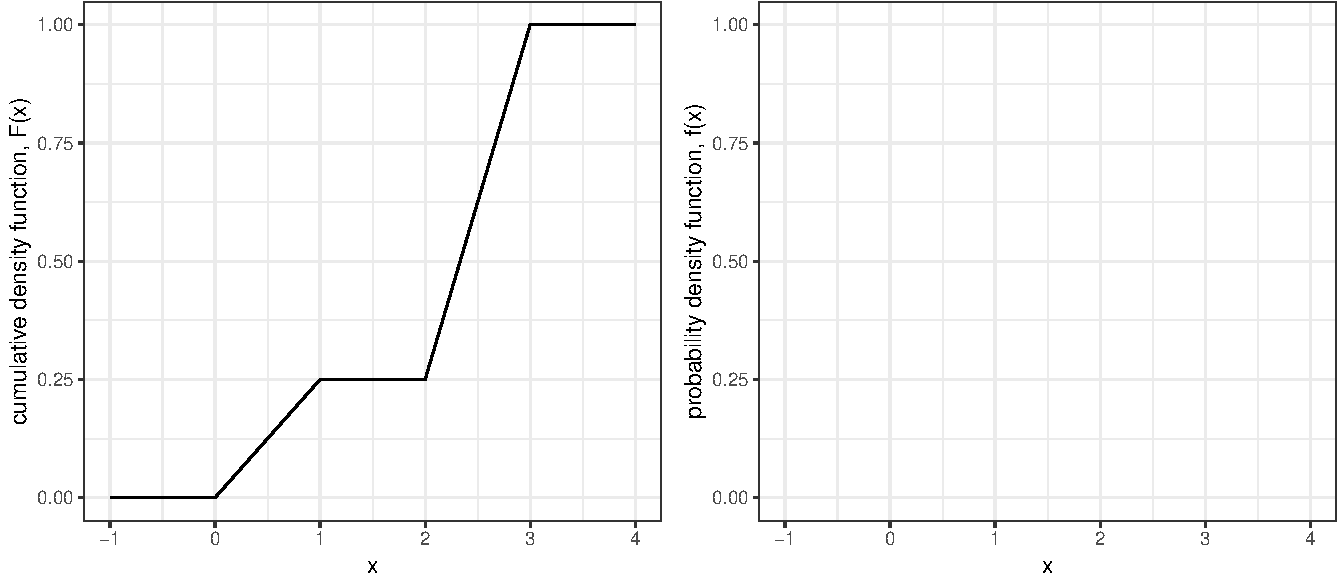
\includegraphics[width=0.9\linewidth,height=.4\linewidth]{stat305-exam2_files/figure-latex/unnamed-chunk-5-1} \end{center}

\vspace{1cm}

\question Suppose \(X\) is a discrete random variable with following
probability function:
\[f(x) = \begin{cases} 0.1 |x| + 0.08 & x = -2, -1, 0, 1, 2 \\ 0 & o.w. \end{cases}\]

\qparts{
\part[2] Find $E(X)$ \vspace{2.5cm}
\part[2] Find $P(|X| = 2)$ \vspace{2.5cm}
\part[2] Find $P(X \ge 0)$ \vspace{2.5cm}
}

\newpage

\question

Let \(X\) be a binomial random variable with \(n = 6\) and \(p = 0.2\).
\qparts{
\part[2] Find $P(X = 3)$ \vspace{2cm}
\part[2] Find $P(X > 4)$ \vspace{2cm}
\part[2] Find $E(X)$ \vspace{2cm}
\part[2] Find $Var(X)$ \vspace{2cm}
}

\question

Suppose \(Y\) is an exponential random variable with \(E(Y) = 2\).
\qparts{
\part[2] Find $P(Y \le 3)$ \vspace{2cm}
\part[2] Find $P(1 \le Y \le 3)$ \vspace{3cm}
\part[2] What is the cumulative density function of $Y$ \vspace{3cm}
\part[2] Find $Var(Y)$ \vspace{2cm}
}

\newpage

\question

Let \(X\) be a normal random variable with a mean of 50 and a varaince
of 25 (i.e., \(X \sim N(50, 25)\)) and let \(Z\) be a random variable
following a standard normal distribution. Find the following
probabilities (note: the Standard Normal Probabilites table attached at
to the exam will helpful): \vspace{1cm} \qparts{
  \part[2] $P(Z > 0.1)$ \vspace{2cm}
  \part[2] $P(|Z| \le 1.25)$ \vspace{2cm}
  \part[2] $P(1 < Z < 3)$ \vspace{2cm}
  \part[2] $P(X < 40)$ \vspace{3cm}
  \part[2] $P(|X-50| \le 12.5)$ \vspace{3cm}
  \part[5] Find the value $a$ so that $P(X > a) = 0.85$
}

\newpage

\question

We are going to play a game involving four bags. The first bag contains
10 lettered wooden tiles (3 letterd A, 2 lettered B, and 5 lettered C).
The other bags are labelled \textbf{Bag A}, \textbf{Bag B},
\textbf{Bag C} and contain the following:

\qitems{
\item \textbf{Bag A}: 25 colored marbles: 16 Blue, 4 Red, 3 Green, and 2 Yellow.
\item \textbf{Bag B}: 50 colored marbles: 10 Blue, 38 Red, 1 Green, and 1 Yellow.
\item \textbf{Bag C}: 30 colored marbles: 1 Blue, 11 Red, 17 Green, and 1 Yellow.
}

Once you have learned the contents of the bags, we play the following
game:

\qitems{
\item First, I randomly select a tile from the bag of tiles (you do not see the tile). 
\item Next, I take the bag of marbles with the label matching the letter on my tile (you do not see which bag I take).
\item Then, I randomly select a marble from the bag I took.
\item Finally, I show you the marble. 
}

You win the game by correctly guessing the letter on the tile I drew.
\vspace{.3cm}

\qparts{
\part[2] What is the probability that I start the game by drawing a tile with the letter A? \vspace{3cm}
\part[2] What is the probability that I draw a blue marble \textit{given} that I drew a tile with the letter A? \vspace{3cm}
\part[2] What is the probability that I start the game by drawing a tile with the letter A and then draw a blue marble? \vspace{3cm} 
\part[2] What is the probability that I start the game by drawing a tile with the letter C and then draw a blue marble? \vspace{3cm} 
\part[2] What is the probability that the marble I show you a blue marble? \vspace{3cm}
\part[2] What is the probability that I drew a tile with the letter A \textit{given} that I show you a blue marble? \vspace{3cm}
\part[2] What is the probability that I drew a tile with the letter B \textit{given} that I show you a green marble? \vspace{3cm}
}

\newpage

\question

Suppose that \(X\) is a continuous random variable with probability
density function (pdf):
\[ f(x) = \begin{cases} c(4 - x^2) &  -2 \le x \le 2 \\ 0 & \text{otherwise} \end{cases} \]
where \(c\) is a constant (not necessarily positive).

\qparts{
\part[2] What is the value of $c$ if $f(x)$ is a valid probability density function? \vspace{3cm}
\part[5] Sketch the probability density function using the grid below (including the points $(-2, f(2))$, $(0, f(0))$, and $(2, f(2))$).


\begin{center}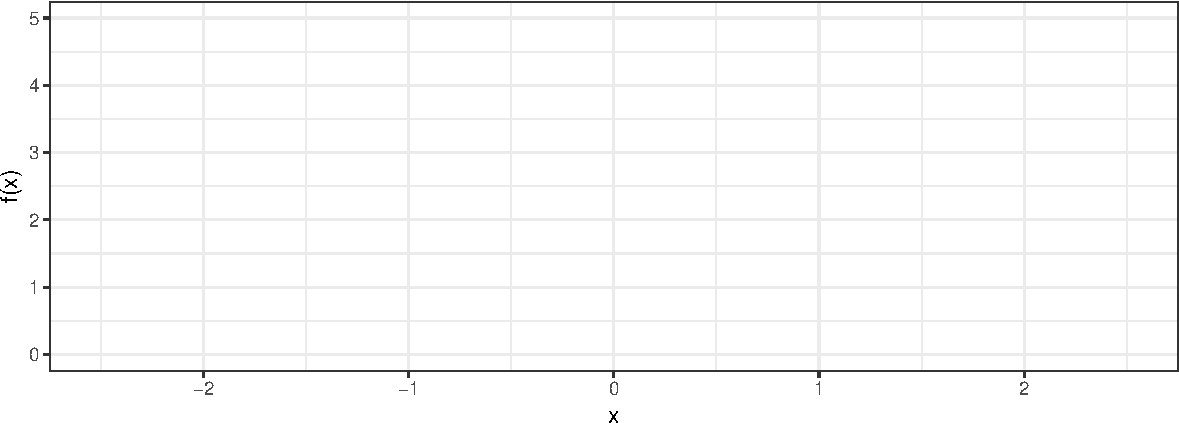
\includegraphics[width=0.8\linewidth,height=0.3\linewidth]{stat305-exam2_files/figure-latex/unnamed-chunk-6-1} \end{center}
\part[4] What is the cumulative density function, $F(x)$? \vspace{3.5cm}
\part[2] What is the probability that $X$ takes a value greater than 0.5? \vspace{2cm}
\part[2] What is the probability that $X$ takes a value between 0.5 and 1? \vspace{2cm}
}

\end{questions}

\end{document}
